%%%%%%%%%%%%%%%%%%%%%%%%%%%%%%%%%%%%%%%%%%%%%%%%%%%%%%%%%%%%%%%%%%%%%%
% LaTeX Example: Project Report
%
% Source: http://www.howtotex.com
%
% Feel free to distribute this example, but please keep the referral
% to howtotex.com
% Date: March 2011 
% 
%%%%%%%%%%%%%%%%%%%%%%%%%%%%%%%%%%%%%%%%%%%%%%%%%%%%%%%%%%%%%%%%%%%%%%
% How to use writeLaTeX: 
%
% You edit the source code here on the left, and the preview on the
% right shows you the result within a few seconds.
%
% Bookmark this page and share the URL with your co-authors. They can
% edit at the same time!
%
% You can upload figures, bibliographies, custom classes and
% styles using the files menu.
%
% If you're new to LaTeX, the wikibook is a great place to start:
% http://en.wikibooks.org/wiki/LaTeX
%
%%%%%%%%%%%%%%%%%%%%%%%%%%%%%%%%%%%%%%%%%%%%%%%%%%%%%%%%%%%%%%%%%%%%%%
% Edit the title below to update the display in My Documents
%\title{Project Report}
%
%%% Preamble
\documentclass[paper=a4, fontsize=11pt]{scrartcl}
\usepackage[T1]{fontenc}
\usepackage{fourier}

\usepackage[english]{babel}                                                         % English language/hyphenation
\usepackage[protrusion=true,expansion=true]{microtype}  
\usepackage{amsmath,amsfonts,amsthm} % Math packages
\usepackage[pdftex]{graphicx}   
\usepackage{url}
\usepackage{pstricks-add}
\usepackage{pgfplots}
\usepackage{listings}

%%% Custom sectioning
\usepackage{sectsty}
\allsectionsfont{\centering \normalfont\scshape}


%%% Custom headers/footers (fancyhdr package)
\usepackage{fancyhdr}
\pagestyle{fancyplain}
\fancyhead{}                                            % No page header
\fancyfoot[L]{}                                         % Empty 
\fancyfoot[C]{}                                         % Empty
\fancyfoot[R]{\thepage}                                 % Pagenumbering
\renewcommand{\headrulewidth}{0pt}          % Remove header underlines
\renewcommand{\footrulewidth}{0pt}              % Remove footer underlines
\setlength{\headheight}{13.6pt}


%%% Equation and float numbering
\numberwithin{equation}{section}        % Equationnumbering: section.eq#
\numberwithin{figure}{section}          % Figurenumbering: section.fig#
\numberwithin{table}{section}               % Tablenumbering: section.tab#


%%% Maketitle metadata
\newcommand{\horrule}[1]{\rule{\linewidth}{#1}}     % Horizontal rule

\title{
        %\vspace{-1in}  
        \usefont{OT1}{bch}{b}{n}
        \normalfont \normalsize \textsc{} \\ [25pt]
        \horrule{0.5pt} \\[0.4cm]
        \huge CSE 221 Final Project \\
        \huge       Draft 2         \\
        \horrule{2pt} \\[0.5cm]
}
\author{
        \normalfont                                 \normalsize
        Patrick Bird\\[-3pt]        \normalsize
        patbird@gmail.com\\           \normalsize
        \today
}
\date{}


%%% Begin document
\begin{document}
\maketitle
\section{Introduction}
Over the last decade, an increasing number of services are transitioning to the cloud to leverage some of its power.  Pre-configured virtual machines and unlimited object storage attract many an organization.  Many of these services attract companies who do not want to invest time and money into supporting infrastructure that is not in their area of specialty.

The area of big data is also an interest to many.  Many organizations and instutions are amassing large datasets that is challenging on one hand and frightening on another.  It's exciting since there is much potential to learn new connections between data that wasn't known before.  But it is also crippling from not knowing where to start analyzing and drawing connections.

With both cloud technology and big data as dominant technological forces, the infrastructure is crtical for maintaining a robust platform to explore these two areas of technology.  The institution where I work in is involved in these two areas and that is what has motivated me to understand and characterize a portion of that system.

The current work project that I work on, basespace.com, leverages Amazon AWS services such as EC2, S3, SQS, and more.  And since our product is mainly the analysis of genomic data, the need for high throughput of data, compute, and parallelism is needed.  Many of our data analyses can take several hours to compute.  This timespan may seem acceptable, but as genomics and the clinical lab converge, speed will be critical for diagnosing health issues.

Focusing on cloud computing, I wanted to characterize a local, high-performance bare-metal compute node.  Although outside the scope of this paper, I would eventually like to extend the study to actual VMs on these compute nodes and to compare their performance with the bare metal.  For instance, how does an 8 VCPU virtual machine with 64 GB of memory compare with its bare-metal constituents.  What would be the cost of virtualization?

Since this study involves high performance time measurement, I wanted to get as close as I could to the hardware without writing the whole thing in assembly.  Not to mention, the node runs CentOS linux, and knowing that GCC and the standard POSIX C headers were readily available, no other languages were really considered.  No special compiler options were really used either.  The only options I needed to provide were to link in math libraries for calculating the square root and for using pthreads.

So far, I have invested about 30 hours into this project thus far.  I alone have done all the work in both research, code implementation, and the production of this paper.

\section{Machine Description}

The system has two processors, with each having six cores that are hyperthreaded.  This information was called from /proc/cpuinfo and matched with the information from Intel's website.  The processors are Intel Xeon E5-2620 that run at 2000.053 MHz to be exact.  There are three levels of cache - 32 KB of L1 each for data and instructions, 256 KB of L2 (both), and 15,360 KB of L3 (both).  The instruction pipeline is anywhere from 17 to 20 stages.

The memory size is 128 GB of DDR3 RAM.  The potential speed is 1600 MHZ, however due to the fact that the processor can at max handle 1333 MHz, the configurable clock speed is set to 1333 MHz.  The processor is setup so that it can utilize four memory channels with the RAM.  The more channels it has, the greater opportunity the processor has for read and write parallelism.  This information was found by the dmidecode command.

The hard disk is a 1 TB hard disk drive at 7200 RPM.  The network card is full duplex gigabit ethernet.  The operating system is 64-bit CentOS v6.4, kernel version v2.6.32-358.11.1.

\section{Operations}
This section will describe various machine operations, how I estimated performance on them, and how I performed measurements to measure these operations and their corresponding results.  To begin with, this system is not a single RISC processor.  Unfortunatley for my current purposes, but to my computer's delight, there is not a one to one mapping between instructions and clock cycles.  At least for the first few operations, I couldn't merely just count up the instructions and add a little for overhead.

As I mentioned in Section 2, these processsors have multi-cores three levels of cache, and a 17-20 stage pipeline, with an interprocessor communication mechanism.  Needless to say, estimating any sort of operation is difficult without an exhaustive knowledge of the internals of the processor and the system.  And even then, the estimation would still only be a ballpark figure.

Since there are so many variables in the system, I wanted to set out and eliminate as many as I could before I started to measure.  For one, I wanted to bind this measurement process to a particular processor.  If my process was interrupted and switched out to a different one, I wanted to ensure that the clock that I read every time was from the same processor.

Thus, one of the first things that my process does upon startup is to set processor affinity.  There is a POSIX routine for this called \textit{sched\_setaffinity}.  When this routine is run at the beginning of my process, the process binds itself to the first processor.  With this binding, at least my clock will not vary from jumping to different CPUs.

My next goal was to elevate the priority of the process to limit context switching as much as possible.  Obviously, I wouldn't have full control over how much CPU bandwidth I could use.  Again, there is a POSIX procedure for setting the priority - \textit{setpriority}.  This process is elevated to the minimum nice value, which is the highest priority.  At this point in time, it is -20.

Both of these decisions did not come easily.  The main drawback was that the typical use case would be eliminated, at least for the time being.  When performing measurements, it is good to know what the measurement would be for typical scenearios instead of highly optimized ones.  However, what caused me to decide to bind to a processor and elevate the process' priority was again the effort to eliminate as many variables as I could.  My reasoning was that these variables can always be reintroduced later if they needed to be measured.

All the measurements are in clock cycles.  However, a simple formula exists to calculate the time that operation took:

\begin{gather}
time(s)=cycles/2,000,000,000 Hz
\end{gather}


\subsection{Measurement Overhead}

How time is measured for performance metrics such as this paper is one of the more fundamental mechanisms.  Every measurement will be built on how time is measured.  And since the system is incredibly complex, measuring time is a difficult process.  One of the first decisions that needed to be made was whether to count clock cycles or to measure time through some sort of native timestamp.

At least to begin with, some of the operations were quite small which warranted the granularity of the clock cycle.  Any library call that would get the calendar time would need to have some extra code to translate the real time clock to a data structure.  This translation would add yet another cost to understanding the true overhead of the system.

Thus, \textbf{RDTSC} seemed to be the operation to go.  It is one instruction on this chipset, which would read the real time clock of the CPU.  And it is not a privleged call, so there is no overhead in reading it.  However, as I read more about the instruction and the CPU, I understood that the CPU is out of order processor.  Thus, there is no guaranteee when a certain instruction will execute.  To put it in other words, one cannot just look at the assembly and trust that the processor will execute it sequentially.  This processor has almost twenty stages in its pipeline.

Thus, there needed to be a way to serialize the calls, or create an instruction barrier.  \textbf{CPUID} seemed to be a favorite instruction to call right before \textbf{RDTSC} since it is a serializing call.  Unfortunately, this instruction comes with somewhat of a performance penalty.  Thankfully, I came across \textbf{RDTSCP}, which is a serializing \textbf{RDTSC} call.

\subsubsection{Estimation}

After the small routine to read the clock is loaded into cache, there is not much hardware interaction other than the CPU itself.  Since this is the case, a hardware estimation includes examining the software routine for performance.  There are fifteen assembly instructions in the \textit{GetRdtscp()} procedure with another four instructions for calling and returning.  In all, there about twenty instructions.  Accounting for 20\% overhead, my hardware estimation is 24 clock cycles.

The operating system does not add much overhead in this operation.  After the instructions are loaded from memory, the instructions will most likely stay in cache.  Thus, another 20\% overhead will be accounted for random context switching.  Thus, the overall estimation time is around 30 clock cycles (15 ns).

\subsubsection{Measurement}

After running the experiment a 1000 times, I get the following results:

\begin{center}
    \begin{tabular}{ | l | l | l | l |}
    \hline
    Hardware Estimate & Software Estimate & Total Estimate & Measurement \\ \hline
    24 cycles & 5 cycles & 30 cycles & 35 cycles (18 ns) \\ 
    \hline
    \end{tabular}
\end{center}

My estimation was actually not as bad as I expected it to be.  My estimation was faster than what the average speed of the routine was, but close enough.  In fact, my estimation matched the minimal value that I observed over 1000 iterations.  Part of the reason why I think my estimate was fairly good was that there was not much happening here as far as the system goes.  There is no outside interface with peripheral devices or memory for that matter.

The memory issue is interesting because for the most part, my performance only took a hit during the first iteration.  The CPU had to fetch the procedure from memory and load it into its cache.  After the routine was in cache, the performance increased significantly.

As one can observe by the next grid, there is a tight range between the min and the max.  There is only a difference of 11 clock cycles with a standard deviation of 2.68 clock cycles.  The max in the table lists the max other than the first data point.  I intentionally did this for two reasons.

\begin{center}
    \begin{tabular}{ | l | l | l | l | l | l |}
    \hline
    No. of Samples & First Iteration & Min & Max (excluding 1st) & Mean & Standard Deviation \\ \hline
    1000 iterations & 53 cycles & 30 cycles & 41 cyles & 35.0 cyles & 2.68 cycles \\ 
    \hline
    \end{tabular}
\end{center}

For one, in all my measurements, I want to observe the cost of the CPU fetching the routine from memory if it has not already done so.  I also wanted to know after that, what is the next maximum value.  I followed this process for each of the operations.

\subsection{Loop Overhead}

\subsubsection{Estimation}

Adding a loop construct to the measurement routine does not introduce a heavy burden.  In reality, it is just a few more instructions to add to the measurement routine.  And since it is a loop, there is pointer arithemetic that needs to happen to store the clock value.  Again there is no significant operating system cost to account for, so the entire extra cost for a loop routine will fall in the hardware domain.  Using the average cost from the RDTSCP routine, I estimate that the cost for a loop will be an extra ten cycles based upon the additional hardware instructions or 38 clock cycles (19 ns).

\subsubsection{Measurement}

After running the experiment a 1000 times, I observe the following results:

\begin{center}
    \begin{tabular}{ | l | l | l | l |}
    \hline
    Hardware Estimate & Software Estimate & Total Estimate & Measurement \\ \hline
    33 cycles & 5 cycles & 38 cycles & 47 cycles (24 ns) \\ 
    \hline
    \end{tabular}
\end{center}

The estimate was actually very close to the actual answer which is very pleasing.  Though, trying to estimate this routine from scratch would have been much more difficult.  Since I had the convienence of the previous metric, my estimate was able to be close to the measured value.

\begin{center}
    \begin{tabular}{ | l | l | l | l | l | l |}
    \hline
    No. of Samples & First Iteration & Min & Max (excluding 1st) & Mean & Standard Deviation \\ \hline
    1000 iterations & 45 cycles & 45 cycles & 371 cycles & 35.0 cycles & 2.68 cycles \\ 
    \hline
    \end{tabular}
\end{center}

\subsection{Procedure}

\subsubsection{Estimation}

The cost of calling a procedure will most likely be on par with the loop construct.  In the loop construct, there is a branch, an update to a register value, and pointer arithmetic for both the lower and upper 32 bits of the clock value.  For a procedure, it will be pushing and popping registers off the stack.  Obviously, the greater number of arguments, the greater number of registers that need to be pushed and popped.

For zero arguments, there is almost no cost to calling a function other than pushing the return address and the call instruction itself.  For one argument, a register needs to be pushed, and the stack pointer needs to be adjusted.   Also, there is the call instruction. Then, for every variable, an additional register is pushed onto the stack.  Thus, we can use the equation

\begin{align}
clocks& =RDTSCP + 2 + 2n\\
clocks& =2n + 37
\end{align}

Here is a graph of clock cycles against number of arguments.

\begin{center}
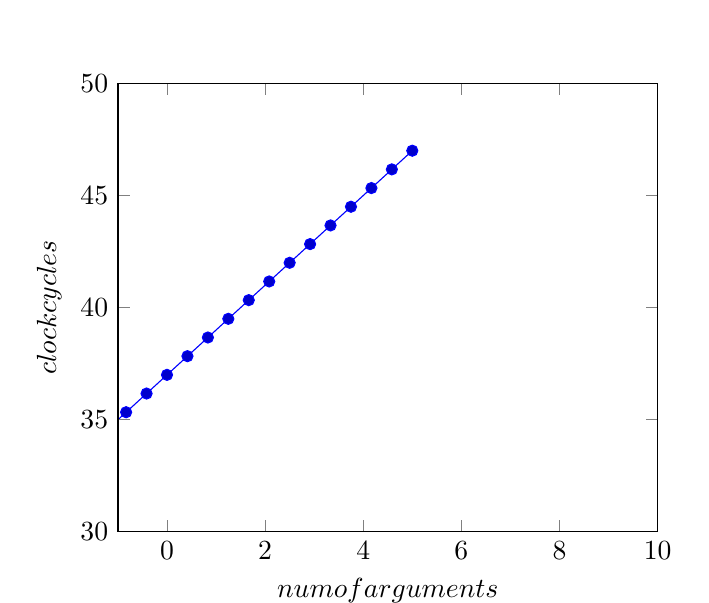
\begin{tikzpicture}
  \begin{axis}[ 
    xmin=-1, xmax=10,
    ymin=30, ymax=50,
    xlabel=$num of arguments$,
    ylabel={$clock cycles$},
    axis on top=true
  ] 
    \addplot {2*x + 37}; 
  \end{axis}
\end{tikzpicture}
\end{center}

In the C routines themselves, I ensured that the arguments were being referenced so the compiler would not try to optimize them away.

\subsubsection{Measurement}

Again, stepping on the shoulders of the RDTSCP measurement has been beneficial.  The measurements are within the bounds of my estimation.

\begin{center}
    \begin{tabular}{ | l| l | l | l | l |}
    \hline
    Argument Count & Hardware Estimate & Software Estimate & Total Estimate & Measurement \\ \hline
    0 & 37 cycles & 5 cycles & 43 cycles & 37 cycles (24 ns) \\ \hline
    1 & 39 cycles & 5 cycles & 44 cycles & 38 cycles (24 ns) \\  \hline
    2 & 41 cycles & 5 cycles & 46 cycles & 40 cycles (24 ns) \\  \hline
    3 & 43 cycles & 5 cycles & 48 cycles & 40 cycles (24 ns) \\  \hline
    4 & 45 cycles & 5 cycles & 50 cycles & 41 cycles (24 ns) \\  \hline
    5 & 47 cycles & 5 cycles & 52 cycles & 40 cycles (24 ns) \\  \hline
    6 & 49 cycles & 5 cycles & 54 cycles & 42 cycles (24 ns) \\ 
    \hline
    \end{tabular}
\end{center}

It is interesting to note that functions with two, three, four, and six arguments had the same average cost of 40 clock cycles.  Not to mention that all eight enumerations of functions are within five clock cyles of each other.  So in some ways there is a linear relationship between additional arguments and the time cost.  However, the cost is neglible.

The various metrics for the different function calls are enumerated here:

\begin{center}
    \begin{tabular}{ | l | l | l | l | l | l | l |}
    \hline
    Arg COunt & No. of Samples & First Iteration & Min & Max & Mean & Std Dev \\ \hline
   0 & 1000 iterations & 89 cycles & 30 cycles & 44 cycles & 37.0 cycles & 4.14 cycles \\ 
    1 &    1000 iterations & 65 cycles & 30 cycles & 44 cycles & 38.0 cycles & 3.2 cycles \\ 
     2 &       1000 iterations & 142 cycles & 33 cycles & 44 cycles & 41.0 cycles & 4.40 cycles \\ 
       3 &         1000 iterations & 68 cycles & 33 cycles & 47 cycles & 40.4 cycles & 3.11 cycles \\ 
        4 &            1000 iterations & 137 cycles & 33 cycles & 47 cycles & 40.9 cycles & 4.23 cycles \\ 
          5 &              1000 iterations & 145 cycles & 36 cycles & 47 cycles & 41.3 cycles & 4.25 cycles \\ 
             6 &               1000 iterations & 68 cycles & 36 cycles & 181 cycles & 40.78 cycles & 5.87 cycles \\ 
              7 &                  1000 iterations & 68 cycles & 36 cycles & 181 cycles & 42.64 cycles & 2.81 cycles \\ 
    \hline
    \end{tabular}
\end{center}

\subsection{System Call}

\subsubsection{Estimation}

For a system call, linux needs to trap into the OS. Thus, there is a heavier cost for a system call as opposed to a user call.  The same registers are pushed onto the stack as a user call.  But there also needs to be some sort of interrupt that happens and an elevation of privleges.  After the user function makes a system call,  the kernel traps into its own routine and takes over.  The kernel then figures out which system call to route to and saves all relevant user state so when it is done, it can transfer control flow back to the user process.  Within the system call itself will copy any releveant user data to its own address space and perform its operation.  After the work is finished, the kernel transfers control flow back to the user process.

The system call is much more expensive than a normal function call because of the elevation of privleges.  Not to mention, there is more copying of data from user space to kernel space and back again.  And there is more state to save.

In the case of a system call, there is more overhead in the operating system than hardware.  As far as hardware is concerned, the CPU will most likely have to fetch the procedure from kernel's address space when it needs to be loaded.  Since system calls happen fairly often, a lot of the instruction data will most likely already be in cache.  But this cost is very similar to a procedure in user space.  It is just in a different place in memory.  Thus, the hardware cost is the base from a user function call - 37 clock cycles.

However, there is a greater cost to the OS here.  In my case, I will measure \textit{getpid()}.  There are at least seven different stages enumerated for this system call.  For each stage, I added an estimate.



\begin{tabular}{ |l|l| }
  \hline
  \multicolumn{2}{|c|}{OS Cost} \\
  \hline
  10 cycles & User state is saved \\
  20 cycles& Elevation of privleges \\
  10 cycles& System function called \\
  10 cycles& Any user data that is needed is copied into kernel space with correct privleges \\
  20 cycles& System call executes \\
  10 cycles& Execution is restored to user \\
  \hline
  80 cycles& total \\
  \hline
\end{tabular}


In all, I estimate about 100 clock cycles will happen just for the operating system part of the system call.  Adding to the hardware cost, I estimate that a system call will take about 117 clock cycles.

\subsubsection{Measurement}

This measurement is the first measurement where I was somewhat dramatically different than the estimation.  In fact, other than the very first call, which took 2427 clock cycles, the average call was a measly 42 clock cycles.  The minimum was 36!  This cost is barely above the user call.  One reason for this large disparity is most likely the efficiency of \textit{getpid()} itself.  The function does not probably take as long to execute at all.  It probably just looks up the address of the calling process in some memory mapped table.  Also, the transfer from user to kernel and back again is much faster than I had assumed.  Again, the address of the procedure must be executed right after the elevation of privleges.  And since no substantial user data needs to be copied, \textit{getpid()} is fairly efficient.

\begin{center}
    \begin{tabular}{ | l | l | l | l |}
    \hline
    Hardware Estimate & Software Estimate & Total Estimate & Measurement \\ \hline
    37 cycles & 100 cycles & 137 cycles & 42 cycles (21 ns) \\ 
    \hline
    \end{tabular}
\end{center}

The following statistical metrics are here.  Notice the cost of the initial call.

\begin{center}
    \begin{tabular}{ | l | l | l | l | l | l |}
    \hline
    No. of Samples & First Iteration & Min & Max (excluding 1st) & Mean & Standard Deviation \\ \hline
    1000 iterations & 2427 cycles & 36 cycles & 83 cycles & 42.41 cycles & 75.51 cycles \\ 
    \hline
    \end{tabular}
\end{center}


\subsection{Task Creation}

\subsubsection{Estimation}

For task creation, there are two main different implementations to take advantage of in linux - processes and pthreads.  The former is invoked using \textit{fork()} where a new process will be created by its parent.  And the two will continue to share memory until a copy-on-write occurs.  This happens whenever one of the processes writes to a shared variable.  Now each process will have its own copy.

A pthread on the other hand uses the \textit{pthread\_create()} function.  Here, there are two threads that share the same memory.  Synchronization is done with atomic shared memory objects like mutexs and condition variables.

The hardware cost for forking a process will mostly be driven by any memory that needs to be copied from the parent to the child.  And it also involves updating any of the parent's address space.  Thus, the cost of creating a new address space for the child is the most significant cost.  Updating several of pages might take a good tens of thousands of clock cycles since the TLBs and cache need to be updated and the permissions need to be copied appropriately.  The cost of hardware is estimated to be 50,000 clock cycles.

From an operating system perspective, the kernel needs to create the process, assign it a new ID, and initiate the copying of any data.  After copying the data, it needs to initiate any updates in the parent.  This management could take a bit of time especially if it is blocked by hardware.  The relative cost of these operations is set at 20000 clock cycles.  In total, I estimate about 70000 clock cycles.

As far as pthreads are concerned, the cost will probably not be as high since memory does not need to be copied over.  Thus, the hardware cost is probably around 10000, just in case any new memory needs to be referenced.  There is not much hardware cost since everything happens more at the kernel level.  The OS will handle the creation of the thread, checking its arguments are valid, and register a new thread at the kernel level.  Since the hardware cost is somewhat neglibile, the kernel cost will be about 10000 clock cycles. 

\subsubsection{Measurement}

Again, the estimates were off by a good bit for processes.  The estimate for threads were a little closer.  This discrepency has probably to do with understanding fork at the hardware level and what all that needs to be copied.  For threads, most of that is managed in software so the cost can be understood a little more.

\begin{center}
    \begin{tabular}{ | l | l | l | l | l |}
    \hline
    Type & Hardware Estimate & Software Estimate & Total Estimate & Average Measurement \\      \hline
    Process & 50,000 cycles & 20,000 cycles & 70,000 cyles & 277,758 cyles (139 us) \\ 
    Thread & 10,000 cycle & 10,000 cycles & 20,000 cycles & 35,443 cycles (18 us) \\
    \hline
    \end{tabular}
\end{center}

The various statistical metrics for these measurements can be found below.  One aspect to notice is that there is a great degree of variance for these measurements.  This fact leads me to believe that memory and disk access has much to play in the cost of creating processes and threads.

\begin{center}
    \begin{tabular}{ | l | l | l | l | l | l |}
    \hline
    No. of Samples & 1st Iteration & Min & Max & Mean & Std Dev \\ \hline
    1000 iterations & 182,993 cycles & 83,727 cycles & 41,948,421 cyles & 277,758 cyles & 2,184,639 cycles \\ 
    1000 iterations & 87111 cycles & 19,804 cycles & 5,901,437 cyles & 35,443 cyles & 197,039 cycles \\ 
    \hline
    \end{tabular}
\end{center}

\subsection{Context Switching}

\subsubsection{Estimation}

The cost for a context switch involves swapping one process or thread out for another.  For processes, the OS needs to manage the synchronization of the processes.  Each OS has its own algorithm for doing so.  Priority and equity rule in this domain.  Just like we saw in the last measurement, the hardware cost for context switching will most likely be driven by the memory/disk cost again.  For instance, if a thread or a process needs to be swapped out, the instructions for the process need to be loaded into the CPU.  If it is a new task, it will most likely have to be retrieved from main memory.

Here, I estimate that thread context switching will be more streamlined than processes because of how threads share memory with one another.  My implementation for measuring the signalling was as follows.  STDIN and STDOUT are opened at the beginning of the  \textit{MeasureForkContextSwitch()} function.  The current process is then forked.  The parent process closes STDIN and call \textit{pause()} to wait for a user signal from its child process.  The child process on the other hand, when started, will close STDOUT, retrieve the timestamp and signal to its parent process.  After signalling, it writes the timestamp to its parent through the pipe.

My implementation for measuring pthread context switching is as follows.  A pthread is created by the main thread.  After creating the thread, the main thread waits on a condition variable.  When the pthread starts, it reads the time stamp value and signals the condition variable.  In the pthread's exit function, it returns the timestamp.  The main thread wakes up when its condition variable and then reads its timestamp.  Afterwards, it joins the other thread and calculates the difference.

The hardware estimate for processes depends on the memory involved and what needs to be swapped in and out.  Threads will be able to leverage more shared memory and not have to swap in and out as often as threads will.  Thus, the hardware estimate for process context switching will most likely be lower than the previous measurement since some of the data will probably be cached.  Thus, my estimate is half of the previous measurement's average which is about 140,000 clock cycles.  The operating system measurement is neglible compared to the hardware.  Thus, the OS estimate will be 10,000 clock cycles.  The total is 150,000 clock cycles.

For threads, the estimate will be lower since it leverages shared memory.  The average from the last measurement is about 35,000 clock cycles.  Thus, I will halve this one as well for memory hardware overhead.  The operating system is not as drastic.  It is involved in managing the condition variable and mutex.  Also, it is responsible for joining the two threads.  Not to mention, the operating system needs to swap one thread into its thread manager and swap the other one out.  The logic involved here might take 10,000 clock cycles.  In all, I estimate that the context switch will take about 45,000 clock cycles.

\subsubsection{Measurement}

The context switching was faster in both cases.  This discrepency is probably due to the fact that the processor was able to cache more of the instructions and data in cache than estimated, which in turn led to less swapping.  Also, the thread management overhead could be more efficient than previously estimated.  The thread context switching is actually extremely efficient compared to the process switching.  Again, this is mainly due to the fact that the threads share the same memory space.

\begin{center}
    \begin{tabular}{ | l | l | l | l | l |}
    \hline
    Type & Hardware Estimate & Software Estimate & Total Estimate & Average Measurement \\      \hline
    Process & 140,000 cycles & 10,000 cycles & 150,000 cyles & 82,674 cycles (41 us) \\ 
    Thread & 35,000 cycle & 10,000 cycles & 45,000 cycles & 3114 cycles (1.6 us) \\
    \hline
    \end{tabular}
\end{center}

The statistical metrics for the various context switching are as follows.  Again, because memory swapping is involved and the TLB needs to be flushed whenever there is a context switch, there is huge variance in the measurements.

\begin{center}
    \begin{tabular}{ | l | l | l | l | l | l |}
    \hline
    No. of Samples & First Iteration & Min & Max & Mean & Std Dev \\ \hline
    1000 iterations & 4,878,939 cycles & 69,176 cycles & 165,570 cyles & 82,674 cyles & 151,883  cycles \\ 
    1000 iterations & 14,667 cycles & 2616 cycles & 19,316 cyles & 3114 cyles & 858 cycles \\ 
    \hline
    \end{tabular}
\end{center}

\section{Memory Operations}

\subsection{Main Memory}

\subsubsection{Methodology}

One of the main challenges about reading from main memory is trying to figure out how to force the process to actually read from main memory.  Since a CPU cache exists, the kernel will attempt to read data into it that it think might be referenced later.  For instance, the first memory operation to be estimated and measured is reading a series of integers from memory.  Creating an array on the heap might bring it into cache upon allocation.  If not initially, it will most assuredly bring it to cache after the first reference.  Along with this value, it could potentially bring its neighboring addresses in too because of locality of reference.  So, another reference to this same spot in memory in the next hundred or so loops will read the value from cache instead of main memory.

So these circumstances pose a couple of problems and they need to be dealt with to accurately measure the different memory entitites.  First of all, when trying to measure main memory, the data structure needs to be of significant size that would make it cumbersome to load the entire thing into the cache.  And second of all, there must be a means of flushing the cache between each measurement to ensure that the next reference will be from memory.

The caches that this system has are 32 KB for L1, 256 KB for L2 and 15 MB for L3.  Thus, I first start by creating a 1 GB static array before any measurements take place.  Having a block of memory this big will give me a greater chance of having the data referenced from main memory.

%To randomly index into the array, I utilize the \textit{rand()} function with the current time as the seed.  Each time I access the random function, I bit XOR it with the previous random number time in order for the pseudo-random number to be based on time\textsubscript{n} and time\textsubscript{n-1}.  So for each read timing, the software randomly calculates an integer offset between 0 and 7,999,996.  The calculations for pseudo-randomness is not part of either the estimation or the final measurement.

%After allocating memory and generating a random index, the first \textbf{RDTSCP} value is read.  Then, the four-byte integer is retrieved from a pseudo-random index in the array.  Then, the \textbf{RDTSCP} is read again.  After this, the memory is freed and the cache is cleared by iterating over a large array to hopefully clear out any lingering data.

After allocating memory, the program steps through array sizes from 2\textsuperscript{8} to 2\textsuperscript{29} array sizes.  Though, one cannot just use a for loop to iterate through the elements since the CPU will leverage spacial locality and bring much of the data in memory.  One needs to stride through the different array sizes.  I utilizted different stride values from 256 to 8192 bytes.  There is a section after the main memory and cache sections that go into the results of striding.

After striding through each, array, the difference is calculated and the measurement is performed 1000 times to calculate an average and other interesting metrics.  One of these metrics is the back-to-back load latency.  Larry McEvoy and Carl Staelin define back-to-back load latency as follows:
\begin{addmargin}[1em]{2em}% 1em left, 2em right
Back-to-back-load latency is the time that each load takes, assuming that the instructions before and after are also cache-missing loads.\footnote{McVoy, L., and Staelin, C.  "lmbench: Portable Tools for Performance Analysis" Proceedings of the USENIX 1996 Annual Technical Conference, January 1996, p. 8.}
\end{addmargin}

To measure the load, I followed the example in the aforementioned paper and created a simple linked list of 1000 nodes.  In the \textit{MeasureBackToBackLoad()} function, the timer is first read and the 1000 item linked list is traversed from begining to end.  After the entire list was traversed, the timer was stopped, and the cache was cleared in the same way as the \textit{MeasureMainMemory()} function.

\subsubsection{Estimation}

As far as estimating both memory latency and back-to-back load latency, the costs will be shared amongst both hardware and software, but the hardware cost will dominate.

In the case of memory latency, the instruction to read the integers from memory will cause the caches to be checked first.  There will hopefully be misses at all three levels, and the data will be fetched from main memory and will most likely be put into L1 cache.

The actual code to read the memory is quite minimal and maybe only a few clock cycles of indexing into an array.  A check and a miss at L1 cache will probably cost 10 cycles.  A check and a miss at L2 will cost around twice that at 20 cycles.  And a check and a miss at L3 will cost 50 cycles.  After that, the CPU will need to fetch from main memory.  There will be some hardware latency to do virtual address translation, which might take around 20 CPU cycles.  Then the read itself because of waiting to refresh might take around 50 cycles.  The read itself will take 10.  All in all, I estimate the hardware cost to be the following

\begin{center}
\begin{tabular}{ l|l }
  10 cycles & L1 Miss \\
  20 cycles & L2 Miss \\
  50 cycles & L3 Miss \\
  20 cycles & Address Translation \\
  50 cycles & Refreshing Cells \\
  10 cycles & Memory Read \\
  \hline
  160 cycles & Total
\end{tabular}
\end{center}

As far as back to back load is concerned, I think the cost will be about 20 cycles greater since the L1 cache lines might still be in the process of being written in.  Thus, I estimate back-to-back load to be about 180 clock cycles.

The kernel is not really involved in the read from main memory.  It is mainly handled by the CPU and MMU.  However, because of uncertaintanties, I will put a cost of 10 clock cycles for the kernel.

The two estimates are:

\begin{center}
    \begin{tabular}{ | l | l | l | l | l |}
    \hline
    Type & Hardware Estimate & Software Estimate & Total Estimate & Average Measurement \\      \hline
    Memory Latency & 160 cycles & 10 cycles & 170 cyles & 206.2 cycles (103 ns) \\ 
    Back-to-back Load & 180 cycles & 10 cycles & 190 cycles & 215.0 cycles (108 ns) \\
    \hline
    \end{tabular}
\end{center}


\subsubsection{Measurement}

To access a single four-byte integer from main memory took on average 206 CPU cycles or 103 ns.  It was somewhat pleasing to see that my estimate was within 30\%.  The max was quite higher at 1550 cycles.  This value could be understood as maybe a short context switch.  The measurements are within a reasonable number for accessing a single integer from main memory.


\begin{center}
    \begin{tabular}{ |l | l | l | l | l | l | l |}
    \hline
    Measurement & \# Samples & First Iteration & Min & Max & Mean & Std Dev \\ \hline
    Memory & 1000 it. & 7642 cycles & 178 cycles & 1550 cycles & 206.2 cycles & 248.1  cycles \\ 
    Back-to-back Load & 1000 it. & 269 cycles & 202 cycles & 317 cycles & 215.0 cycles & 15 cycles \\
    \hline
    \end{tabular}
\end{center}

Measuring the back-to-back load latency was an interesting exercise.  My very first implementation went extremely fast.  It was on the order of 10,000 - 20,000 clock cycles to traverse a 1000 node linked list.  After considering it though, it did not seem that difficult to reason.  All the linked list node structure's definition was a pointer to the next node.  Thus, it was an eight byte field that pointed to the next eight byte field.  When I created the list at the beginning of the program, \textit{calloc()} most likely allocated the memory contiguously.  Thus, reading the list front to back allowed for any locality and readahead optimization by the kernel.  So, in a way, the linked list most likely looked like an array in memory.

So, to take another stab at it, I redefined the structure to include a 50 KB data member.  Adding this field gave my linked list structure more weight which provided for more of a random scattering into memory.  After that, I saw more realistic numbers for back-to-back load.  Although, it was not as costly as either the authors of the lmbench paper or I thought it would be.  In fact, it just added on another 5 clock cycles to the main memory measurement.  After subtracting the loop and timings overheads, the average timing was 215 cycles or 108 ns.  The reasoning for the speedup in back-to-back load could potentially be the fact that cache technology and writes are faster in general than from when the paper was written.

\subsection{L1 \& L2 Caches}

\subsubsection{Methodology}

Trying to force a read from L1 cache is somewhat tricky.  There is no guarantee that the variable that one reads will actually be the one in cache.  However, we can get fairly sure.

To read a integer from L1 cache, I start by reading fifty integers from a static array into L1 cache by way of a \textbf{for} loop.  I could not just define an integer in the function since that would put it in a register.  So, fifty integer are read into L1 cache.  Afterwards, I read \textbf{RDTSCP} and then index to the 25th element of the array.  This element should be in L1 cache.  Then, I read \textbf{RDTSCP} again to find how long the read took.

To read an integer from L2 cache was a little more difficult to figure out than L1.  Somehow, the data I would be referencing would have to be forced out of L1 and drop into L2 without going farther into the L3 cache or back to main memory.  The methodology for forcing a value to L2 continutes where L1 left off.

The L1 size for this machine is 32 KB of data.  It also has 32 KB of instruction cache but that does not pertain to this measurement.  The L2 cache is much larger at 256 KB.  To measure L2, data needs to be read into L1 where it would "spill over" into L2 from where I could read.

A large static two-dimensional integer array (5000x1024) was created for this purpose among others.  All in all, this array measures to be around 20 MB. The \textit{MeasureL2Cache} function randomly indexes into this array and reads 50 different 4 KB blocks (or ~ 200 KB) into the L1 and consequently into the L2 cache.  After these 50 blocks are read in, a random block from the first 30 are indexed into again for the integer read.  The reasoning is that the last 20 blocks will more than cover the 32 KB of L1 cache and that hopefully by reading an integer from the first 30, it will be from the L2 cache. 

\subsubsection{Estimation}

Estimating L1 and L2 cache hits and misses is entirely hardware and not kernel specific.  L1 reads are very fast and will be hardly more than the time it takes to read the \textbf{RDTSCP}.  Thus, I estimate that an L1 hit will take three clock cycles.  L2, on the other hand, will take a good bit longer.  And not just twice as long.  There is an L1 cache miss involved and depending on how far away the L2 cache is, I estimate that L2 will rather take five times as long or about 15 clock cycles.

\begin{center}
    \begin{tabular}{ | l | l | l | l | l |}
    \hline
    Type & Hardware Estimate & Software Estimate & Total Estimate & Average Measurement \\      \hline
    L1 Cache & 3 cycles & 0 cycles & 3 cyles & 10 cycles (5 ns) \\ 
    L2 Cache & 15 cycles & 0 cycles & 15 cycles & 33.8 cycles (16.5 ns) \\
    \hline
    \end{tabular}
\end{center}

\subsubsection{Measurement}

The measurements for the L1 cache estimation.  The average L1 cache read clocked in at 40 clock cycles or 5 more than the \textbf{RDTSCP} call.   Thus, a L1 read took 2.5 ns.  The standard deviation is 3.05 which gives me confidence for my methodology.

The L2 cache measurement was very close to the estimate as well.  The average L2 cache read was 61.9 clock cycles or about 17 clock cycles more than the \textbf{RDTSCP} read.  This timing includes both the L1 miss and L2 hit.  There was more variance in the results (the standard deviation is 48.86) which is mainly due to the fact that it is a little more difficult to force data into the L2 cache.  My guess is that sometimes the data probably went to L3 cache or back to main memory which explains the max read of 506 clock cycles. 

\begin{center}
    \begin{tabular}{ | l | l | l | l | l | l | l |}
    \hline
    Measurement & No. of Samples & First Iteration & Min & Max & Mean & Std Dev \\
    \hline
    L1 Cache & 1000 iterations & 50 cycles & 33 cycles & 50 cycles & 40.84 cycles & 3.05  cycles \\ 
    L2 Cache & 1000 iterations & 57 cycles & 36 cycles & 506 cycles & 61.58 cycles & 48.87  cycles \\ 
    \hline
    \end{tabular}
\end{center}

\subsection{RAM, L1, \& L2 Comparison with Arrays}

As you can see in the below graph, there are steps to indicate both the L1, and L2 caches.  Because of the large amount of cache, we didn't observe a step up until about 2\textsuperscript{23} byte arrays.  This was mainly due to the locality of the striding.  The stride values would often overlap with each other which caused the steps to be seen in values greater than the actual cache values.

Another step up around a 2\textsuperscript{24} array size.  From there, the graph would show L3 and main memory.

\begin{center}
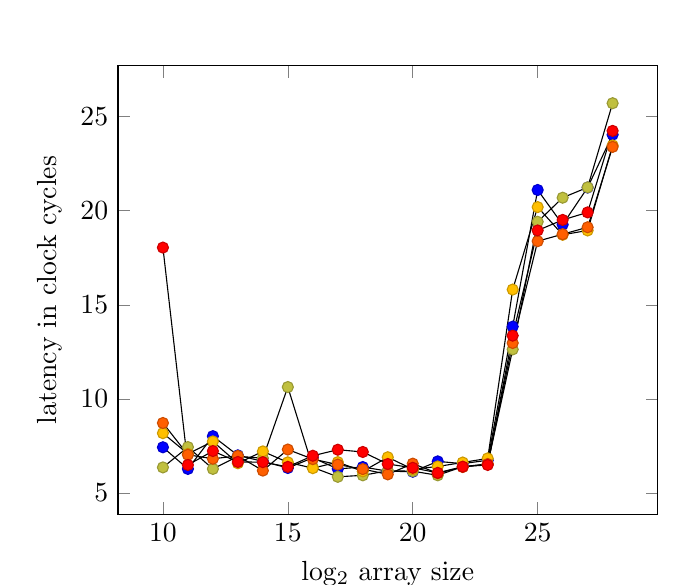
\begin{tikzpicture}[domain=0:3]
\begin{axis}[xlabel={log\textsubscript{2} array size}, ylabel={latency in clock cycles}]
\addplot[scatter, scatter src=\thisrow{class},
      error bars/.cd, y dir=both, x dir=both, y explicit, x explicit, error bar style={color=mapped color}]
      table[x=x,y=y] {
    x       y      class

    10      7.43     0
    11      6.28     0
    12      8.02     0
    13      7.00     0
    14      6.68     0
    15      6.33
    16      6.87
    17      6.28
    18      6.38
    19      6.16
    20      6.13
    21      6.68
    22      6.56
    23      6.74
    24      13.84
    25      21.10
    26      19.26
    27      21.23
    28      24.04
};

\addplot[scatter, scatter src=\thisrow{class},
      error bars/.cd, y dir=both, x dir=both, y explicit, x explicit, error bar style={color=mapped color}]
      table[x=x,y=y] {
    x       y      class
    10      6.36     1
    11      7.44     1
    12      6.28     1
    13      6.95     1
    14      6.85     1
    15      10.63
    16      6.36
    17      5.86
    18      5.94
    19      6.18
    20      6.16
    21      5.94
    22      6.40
    23      6.54
    24      12.63
    25      19.41
    26      20.69
    27      21.24
    28      25.71
};

\addplot[scatter, scatter src=\thisrow{class},
      error bars/.cd, y dir=both, x dir=both, y explicit, x explicit, error bar style={color=mapped color}]
      table[x=x,y=y] {
    x       y      class
    10      8.18     2
    11      7.08    2
    12      7.74     2
    13      6.58     2
    14      7.21     2
    15      6.63
    16      6.32
    17      6.64
    18      6.15
    19      6.90
    20      6.26
    21      6.41
    22      6.62
    23      6.84
    24      15.81
    25      20.19
    26      18.72
    27      18.95
    28      23.47
};

\addplot[scatter, scatter src=\thisrow{class},
      error bars/.cd, y dir=both, x dir=both, y explicit, x explicit, error bar style={color=mapped color}]
      table[x=x,y=y] {
    x       y      class
    10      8.72     3
    11      7.03    3
    12      6.82     3
    13      6.97     3
    14      6.19     3
    15      7.31
    16      6.80
    17      6.51
    18      6.27
    19      5.99
    20      6.56
    21      6.05
    22      6.38
    23      6.54
    24      12.97
    25      18.38
    26      18.75
    27      19.12
    28      23.39
};

\addplot[scatter, scatter src=\thisrow{class},
      error bars/.cd, y dir=both, x dir=both, y explicit, x explicit, error bar style={color=mapped color}]
      table[x=x,y=y] {
    x       y      class
    10      18.04    4
    11      6.49    4
    12      7.23     4
    13      6.65     4
    14      6.64     4
    15      6.39
    16      6.98
    17      7.30
    18      7.18
    19      6.54
    20      6.34
    21      6.07
    22      6.40
    23      6.49
    24      13.36
    25      18.95
    26      19.51
    27      19.91
    28      24.24
};


\end{axis}
\end{tikzpicture}
\end{center}

\subsection{RAM Bandwidth}

\subsubsection{Methodology}

The first, easy to implement function to read and write from memory would be to take a large array and iterate over it with a for loop.  The single instruction inside the loop would either be the read or the write.  Unfortunately, the loop and the branching would cause significant overhead to the measurement.  Even though, there is a previous measurement of the loop cost, I sought out a more efficient approach.

From James Leiterman's book \textit{32\/64-Bit 80x86 Assembly Language Architecture}, he mentions the \textbf{REP STOSQ} and \textit{REP LODSQ} instructions.  The \textbf{STOSQ} and the \textbf{LODSQ} write and read 8-byte strings of bytes to and from memory, respectively.  The \textbf{REP} prefix informs the CPU to repeatedly perform the instruction for a count specified in the \textbf{RCX} register.  Peforming this instruction will streamline the instructions and remove some of the overhead in branching.

Thus, that is what the \textit{MeasureRamRead()} and \textit{MeasureRamWrite()} functions consist.  The \textbf{RDTSCP} calls wrap both the \textbf{REP STOSQ} and the \textbf{REP LODSQ} instructions.

\subsubsection{Estimation}

The memory has a maximum ideal speed of 1600 MHz.  However, because of the current CPU, the clock for the memory is configured to be 1333 MHz. The data bus is 64 bits wide with some additional bits for error code checking.  There are four memory channels per processor.  However, these channels are shared amongst cores and I don't forsee that the one core that my process is attached to will utilize all four memory channels.

For instance, the Intel website\footnote{http://ark.intel.com/products/64594} specifies the maximum memory bandwidth to be 42.6 GB/s.  And this calculation can be figured out easily.  It takes the fastest DDR3 memory it can handle 1333 MHz, multiplies it by the number of memory channels (4) and then by the 8-byte data bus.

However, these memory channels are shared amongst six cores on the processor.  And since this process will only be on one of the cores, it will probably only use one channel.  So my estimation will only be for one of the channels being utilized.

Thus, we can take the maximum memory bandwidth that Intel provided and divide it by the number of channels (4) since our system is configured with DDR3 1333 MHz RAM.  So, the maximum memory bandwidth for one channel is 10.65 GB/s.

The OS should not add too much overhead, but I will include about a 10\% overhead for it and other things.  So, I hope to reach 9.59 GB/s.

\subsubsection{Measurement}

For RAM read and RAM write, I observed the following measurements:

For the data read operation, it took 5,360,451 clock cycles, or about 2.6 ms, to read from the 5000 x 1024 array on average.  The bandwidth for memory read would then be around:

\begin{gather}
bandwidth = 5000 blocks * 1024 elements * 4 bytes * \frac{2,000,053,000 Hz}{5,360,451 cycles} \\
bandwidth = 7.641 GB/s
\end{gather}

For the data write operation, it took 5,344,615 clock cycles, or about 2.6 ms, to write to the 5000 x 1024 array.  Interestingily enough, this is the exact same time as the data read.  For a sanity check, I ran through the experiment multiple times and I get similar results each time.  The data read and data write are extremely close with one another.  Again the standard deviation is quite small ~ 158,450 clock cycles which is 3\% of the average.  The bandwidth would then be:

\begin{gather}
bandwidth = 5000 blocks * 1024 elements * 4 bytes * \frac{2,000,053,000 Hz}{5,344,615 cycles} \\
bandwidth = 7.664 GB/s
\end{gather}

The write and read bandwidth are quite close with one another.  Unfortunately, the bandwidth is still outside my estimate of 9.64 GB/s.  One reason for lower bandwidth is that this process is bound to a particular core.  If there were a method to leverage all cores and write to memory at the same time, there might be a way to get a more optimized speed.  Also, there are many other services running on this computer.  Some of them are quite large - OpenStack Nova Compute, Swift Object Storage, MySQL, Apach Qpid, and a Windows Server VM.  And unfortunately, I do not have the authority to temporarily suspend these services.  Thus, being within 80\% of my estimate is not difficult to reason.

\begin{center}
    \begin{tabular}{ | l | l | l | l | l | l | l |}
    \hline
     & \# of Samples & First Iteration & Min & Max & Mean & Std Dev \\
    \hline
    Read & 1000 iterations & 5,383,306 c. & 5,152,504 c. & 7,387,026 c. & 5,360,451 c. & 212,472 c. \\ 
    Write & 1000 iterations & 4,925,780 c. & 5,142,160 c. & 6,415,861 c. & 5,344,615 c. & 198,980 c. \\ 
    \hline
    \end{tabular}
\end{center}

\subsection{Page Fault}

\subsubsection{Methodology}

To measure a page fault on this machine with 128 GB of main memory, I needed to create a file that's considerably large in the file system.  At least the file would need to be large enough for the kernel not to bring the entire thing into memory.  I also wanted to chose a size large enough so that I could seek to random points in the file and almost guarantee a page fault.

Thus, the first thing that I did to prepare for this measurement is to generate a 300 GB file.  \textbf{fallocate} would be a good candidate to make a large file fast.  Unfortunately, this command only allocates block and marks them as unitialized.  Not to mention, I wanted to be sure that the file had true random data in it.

Thus, I use the \textbf{dd} command to generate a 300GB file with data from \textit{/dev/urandom}.  The command took a while to perform - about 16 hours or so!

After a random 300 GB file was in place, I was fairly sure that most of my calls to the \textit{MeasurePageFault()} function would indeed generate a page fault.  After entering the measure function, I open the file and generate a random seek position from 0 to 300 billion.  Next, the timer starts, and both \textit{fseek()} and \textit{fread()} are called.  Then the timer is read again for the final time.  This function is repeated a 1000 times.

\subsubsection{Estimation}

The hard drives that are mounted at /home are configured in a Dell PowerEdge RAID controller, H710P.  The two 1 TB HDDs are configured in a RAID 1 configuration meaning that disk reads can be performed in parallel for greater throughput.  Since this test is only measuring reading a single page fault, the RAID configuration should not benefit this test.

The hardware cost is the most significant cost to this operation.  The cost of accessing main memory has already been measured to be about 100 ns on average.  The cost for reading from an HDD will be exponentially larger - probably more than 10,000 times more!  So the main memory measurement is just noise for this measurement and will not be considered.

The hard drives are 7200 RPM which is 120 RPS, or once every 8.3 ms.  If the platter has to travel at least half that time on average, it will take roughly 4 ms just for the platter to spin to the right position.  Then there is the cost of moving the head and reading the data, which might be another 2 ms.

As far as the OS cost would go, the OS will need to check the page table.  And after not finding it, it will attempt a system call to read from disk.  Like the main memory observation, the OS time to service a page fault will pale in comparison to the hardware cost involved.  However, for measurment's sake, I will estimate the page fault service time for the OS to be 100 ns or equivalent to the cost of reading from main memory.

Thus, the total estimation and average measurement is:


\begin{center}
    \begin{tabular}{ | l | l | l | l |}
    \hline
    Hardware Estimate & Software Estimate & Total Estimate & Average Measurement \\      \hline
    6 ms & 100 ns & ~ 6 ms & 19.8 million cycles (9.9 ms) \\ 
    \hline
    \end{tabular}
\end{center}

\subsubsection{Measurement}

After running the \textit{MeasurePageFault()} routine, I retrieved the following results:

\begin{center}
    \begin{tabular}{ | l | l | l | l | l | l |}
    \hline
    \# of Samples & First Iteration & Min & Max & Mean & Std Dev \\
    \hline
    1000 iterations & 33.89 M cycles & 15,603 c. & 87.5 M c. & 19.8 M c. & 10.0 M. c. \\ 
    \hline
    \end{tabular}
\end{center}

My estimate was lower than what was measured and at least within the standard deviation of the average.  There was more variance in the data for a page fault compared to the memory bandwidth.  However, it is still somewhat acceptable.

The standard deviation is half of the average.  The minimum value is 15,603 clock cycles which is a measley 7.8 $\mu$s.  This measurement seems to be too long for it to be accessing main memory since is about 80 times the measurement of main memory.  An explanation for some of the shorter reads is that the head and platter could have been in position with some of its data in a disk cache.  So this miminimum time of 7.8 $\mu$s could be more representative of reading from disk when there is little to no seek time and some of the data could already be buffered to read.

The maximum read was an astounding 43 ms.  A perfect storm of circumstances could cause this phenomenon - a full platter rotate with a context switch to boot.  At any rate, it is a good reminder of the cost of reading from disk and that it can really hinder performance.

Compared to accessing main memory, the average cost of reading a single byte from disk is 4835 clock cycles.  This value was calculated by taking the average time and dividing by the page size - 4096 bytes.  A single byte from main memory is 241 cycles / 4 cycles or ~ 60 cycles.  Thus, a single byte from hard disk is on the order of being 80 times more expensive than one from main memory.  






%%% End document
\end{document}